\chapter{Results and Analysis}\label{results}
\section{Introduction}
This chapter presents the results obtained from the development and application of the Integrated Data Repository (IDR) and decision-support dashboard suite described in Chapter \ref{method}. Following construction of the repository, integrated pathway data were analysed to identify operational bottlenecks, assess service demand and capacity, and evaluate the utility of the artefact for supporting operational decision-making. 

Findings are presented according to the research objectives. The chapter begins by summarising repository development and data quality findings before presenting analysis of oncology referrals, radiotherapy operational performance, and end-to-end pathway delays. The chapter concludes by examining the extent to which the developed artefact supports the design principles established in Chapter \ref{method}.

\section{Repository Development Results}
The IDR successfully integrated datasets originating from multiple operational systems including oncology referral register, Patient Administration System (PAS), and the Aria radiotherapy management system. Data were extracted, transformed and loaded into a PostgreSQL-based repository using layered architecture consisting of staging, intermediate and analytical reporting layers. 

Development of the repository identified several previously unrecognised data quality and interoperability challenges. These included duplicate oncology referral records, inconsistent representation of referral episodes, delayed administrative updates, and differences in event definitions between operational systems. 

The use of intermediate integration views allowed business rules to be applied without modifying source data directly. This approach enabled the construction of analytics-ready fact tables capable of supporting operational reporting while preserving auditability and traceability to originating systems. 

The repository subsequently became the single source of truth for all dashboard metrics and pathway analysis. 

\section{Oncology Referral Analysis}

\subsection{Referral Workload}
 Figure \ref{fig:DB_Onc} presents the Oncology Referral Dashboard developed to support management of referral workload, appointment access, and clinic outcome recording. 

 \begin{figure}[htbp]
    \centering
    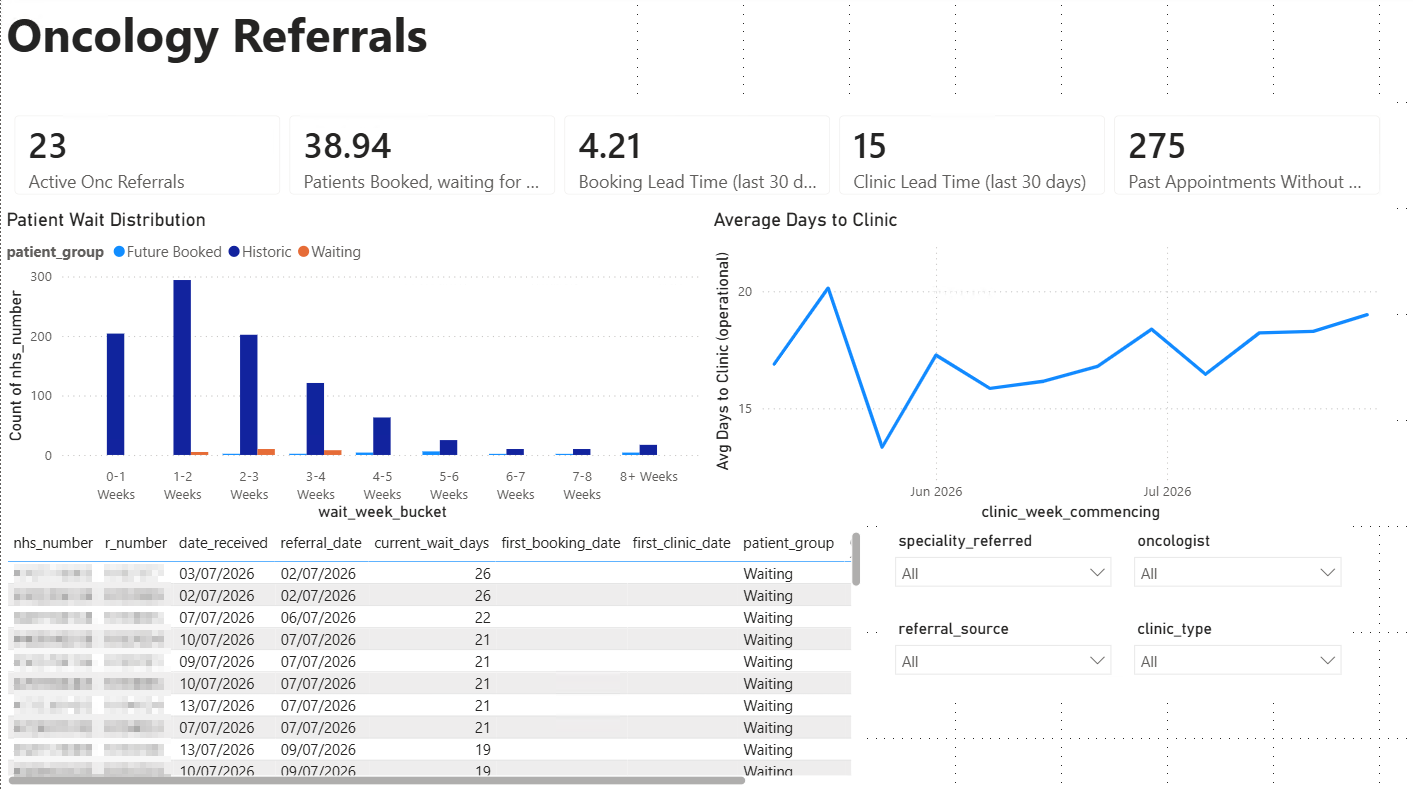
\includegraphics[width=0.85\textwidth]{DB_Onc.png}
    \caption{Operational Oncology Referral Dashboard}
    \label{fig:DB_Onc}
\end{figure}

 Analysis of the oncology referral dashboard identified 23 active oncology referrals at the time of analysis. While this represents a manageable operational workload, variation was observed in waiting times between referral and clinic attendance. 

The distribution of patient waits demonstrated that the majority of patients were clustered within the first three weeks following referral. Smaller numbers of patients remained on the waiting list beyond six weeks, suggesting that the majority of referrals progressed through the booking process relatively efficiently.

\subsection{Booking and Clinic Lead Times}
The average referral-to-booking interval during the previous 30 days was 4.15 days, indicating that referrals were generally triaged and allocated appointments within one working week.

The median referral-to-clinic interval was 15 days. Trend analysis demonstrated that this value remained relatively stable across the observation period, fluctuating between approximately 13 and 20 days.

These findings suggest that initial referral processing and appointment allocation were not the primary sources of pathway delay. The majority of patients received clinic appointments within a timeframe considerably shorter than national cancer waiting-time thresholds.

\subsection{Future Booked Waits}
Patients holding future clinic appointments had an average booked waiting time of 38.94 days. 

This metric should be interpreted carefully, as it does not represent patients awaiting their first oncology appointment following referral. First-appointment access is more accurately reflected by the referral-to-clinic interval, which remained stable at a median of 15 days. 

The future booked wait metric incorporates a broader range of appointment types including routine follow-up appointments, treatment reviews, surveillance activity, and result-discussion clinics. Consequently, the longer waiting time observed is likely to reflect the scheduling characteristics of ongoing oncology care rather than delays affecting newly referred patients. 

Nevertheless, the measure provides useful visibility of future clinic workload and demonstrates demand already committed within existing clinic schedules. This information may assist operational planning by highlighting the volume of future activity competing for available clinic capacity.

\subsection{Incomplete Outcome Recording}
The dashboard identified 275 historical clinic appointments without recorded outcomes. 

This finding represents a significant data-quality issue because pathway progression, attendance analysis, and downstream performance reporting depend upon accurate recording of appointment outcomes. The presence of a large number of unresolved appointments highlights the importance of integrated operational monitoring and demonstrates how the artefact can reveal process weaknesses that may not be visible through conventional reporting. 

\section{Radiotherapy Service Analysis}


\subsection{Operational Workload}

Figure \ref{fig:DB_RT} illustrates the Radiotherapy Service Health Dashboard developed to support monitoring of utilisation, demand forecasting, and patient risk status.

\begin{figure}[htbp]
    \centering
    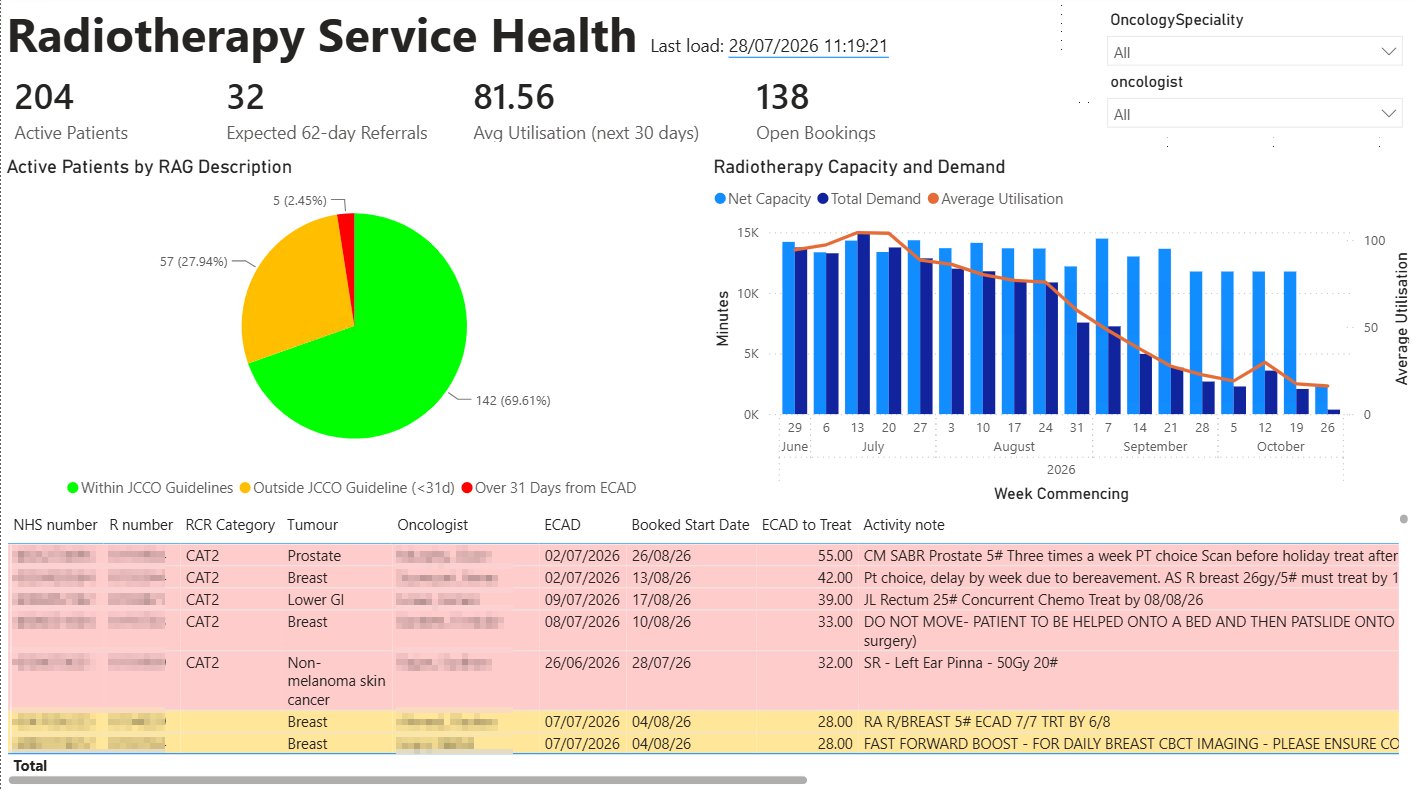
\includegraphics[width=0.85\textwidth]{DB_RT.png}
    \caption{Radiotherapy Capacity and Demand Dashboard}
    \label{fig:DB_RT}
\end{figure}

The radiotherapy dashboard identified 204 active patients undergoing management within the radiotherapy pathway.

In addition, 32 future referrals were predicted to enter the service under a 62-day pathway, defined as oncology referrals booked into Clinical Oncology clinic. This provides operational managers with advance visibility of future demand and supports proactive planning of treatment capacity. 

\subsection{Capacity Utilisation}
Capacity-demand modelling identified an average projected utilisation of 81.56\% across the next 30 days, exceeding the departmental planning threshold of 80\%. This threshold is used operationally to preserve flexibility for urgent treatments, machine downtime, replanning activity, and other unplanned service pressures.

Forecast utilisation declined across the later periods of the planning horizon. However, this reduction should be interpreted with caution because future demand is inherently less complete than near-term demand. The model includes patients currently booked for treatment and referrals that have already entered the radiotherapy pathway, but does not yet reflect patients who have not progressed sufficiently through upstream stages of the pathway. Consequently, the later forecasting periods are likely to underestimate true future demand. 

Despite this limitation, the model provides a useful indication of current service pressure and demonstrates that the radiotherapy service is operating at or slightly above its internal planning threshold.

\subsection{Patient Risk Stratification}
Patient-level risk analysis identified: 

\begin{itemize}
    \item 142 patients (69.61\%) within JCCO guidelines \citep{ash2004}.
    \item 57 patients (27.94\%) outside JCCO guidelines, but within NCWT targets \citep{johnson2024}.
    \item 5 patients (2.45\%) outside the NCWT 31-day standard.
\end{itemize}

Although the majority of patients remained within the recommended timeframes, the presence of patients approaching or exceeding target thresholds demonstrates the value of a proactive monitoring approach.

Rather than identifying breaches retrospectively, the dashboard allows operational teams to focus attention on patients most likely to experience future delays. 

\section{End-to-End Pathway Analysis}


\subsection{Pathway Duration}

Figure \ref{fig:DB_Over} presents the integrated pathway dashboard, combining referral, clinic, and radiotherapy data to visualise pathway progression and identify bottlenecks.

\begin{figure}[htbp]
    \centering
    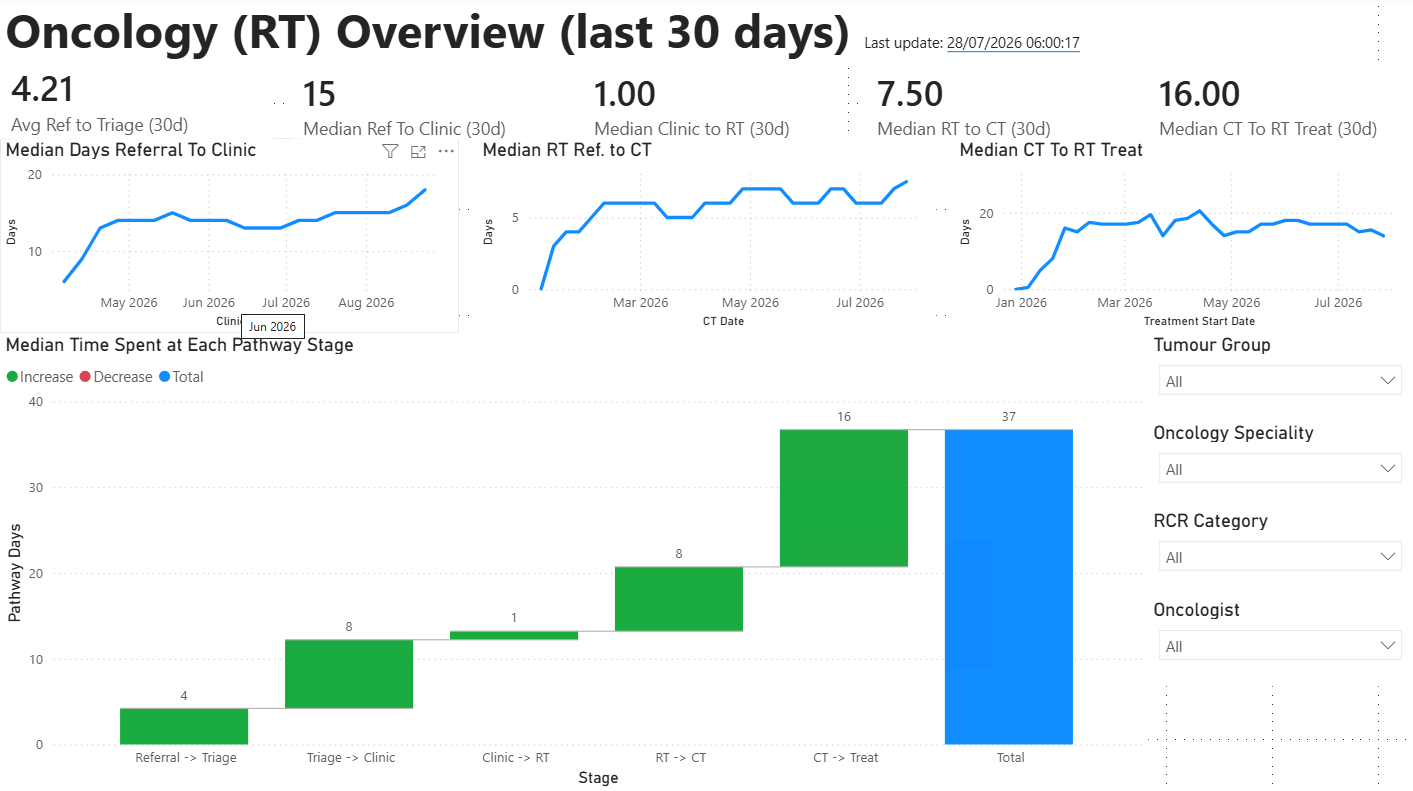
\includegraphics[width=0.85\textwidth]{DB_Overview.png}
    \caption{Integrated Post-MDT Pathway Dashboard}
    \label{fig:DB_Over}
\end{figure}

The integrated pathway dashboard (Figure \ref{fig:DB_Over}) enabled analysis of patient progression from referral through to treatment initiation.

The median pathway duration was 37 days and was composed of five principal operational stages:

\begin{table}[h]
    \centering
    \begin{tabular}{|p{7.5cm}|p{7.5cm}|}
        \hline
        \textbf{Stage} & \textbf{Days} \\
        \hline\hline
        Referral \textrightarrow Triage & 4 \\
        Triage \textrightarrow Clinic & 8 \\
        Clinic \textrightarrow RT Referral & 1 \\
        RT Referral \textrightarrow CT & 8 \\
        CT \textrightarrow Treatment & 16 \\
        \hline
        \textbf{Total} & \textbf{37} \\
        \hline
    \end{tabular}
    \caption{Median duration between canonical events in the Radiotherapy post-MDT pathway}
    \label{tab:path_dur}
\end{table}

\subsection{Bottleneck Identification}
The cumulative waterfall visual shown in Figure \ref{fig:DB_Over} demonstrates the largest delay occurred between CT simulation and treatment commencement, accounting for 16 days of the overall pathway.

The second-largest delay occurred between triage and first clinic attendance, accounting for 8 days.

Together these two stages represented approximately two-thirds of the total pathway duration, suggesting that operational improvement efforts should be concentrated in these areas.

In contrast, the interval between clinic attendance and radiotherapy referral was only one day, indicating that MDT and consultant decision-making processes were not a significant source of delay.

\subsection{Temporal Trends}
Trend analysis demonstrated that:

\begin{itemize}
    \item Referral-to-clinic performance remained relatively stable.
    \item RT Referral-to-CT increased from approximately 0 days to 7 days before stabilising.
    \item CT-to-Treatment remained consistently between 15 and 20 days.
\end{itemize}

The persistence of the CT-to-treatment interval suggests that a substantial proportion of pathway time is spent between CT simulation and treatment initiation. However, this interval represents an aggregation of several planning and preparation activities rather than a single operational process. 

Following CT simulation, patients typically undergo contouring, treatment planning, plan review, quality assurance, and treatment scheduling before treatment can commence. These activities do not currently form part of the canonical pathway events recorded within the repository but nevertheless consume operational time and resources. 

Consequently, further investigation is required before this interval can be interpreted solely as a treatment-capacity issue. Opportunities for future work are discussed in Chapter \ref{discussion}.

\subsection{Research Question 1}
The pathway dashboard directly addressed Research Question 1:

\textbf{Where do delays occur between MDT outcome and treatment?}

Analysis demonstrated that delays are concentrated primarily within:

\begin{enumerate}
    \item CT Simulation \textrightarrow Treatment Start.
    \item Triage \textrightarrow Clinic Attendance.
\end{enumerate}

These stages therefore represent the most significant opportunities for operational intervention. 

\section{Evaluation of Design Principles}

\begin{table}[h]
    \centering
    \begin{tabular}{|p{7.5cm}|p{7.5cm}|}
        \hline
        \textbf{Design Principle} & \textbf{Evidence from Artefact} \\
        \hline\hline
        DP1: Surface Breach Risks & RAG categorisation and patient risk worklists \\
        DP2: Pair Risk with Capacity & Capacity and demand dashboard visualisations \\
        DP3: Canonical Events & Standardised pathway intervals derived from warehouse fact tables \\
        DP4: Refresh Cadence & Automated ETL pipeline and scheduled refresh processes \\
        DP5: Provenance and Auditability & Staging, intermediate and fact-layer architecture with ETL logging \\
        DP6: Task-Oriented Design & Separate referral, radiotherapy and pathway dashboards aligned to operational workflows \\
        \hline
    \end{tabular}
    \caption{Artefact evidence of Design Principles}
    \label{tab:DP-Art}
\end{table}

The evaluation suggests that all six design principles were successfully implemented within the final artefact.

Particularly strong support was observed for DP1 and DP2. Operational users were able to identify patients approaching target breaches while simultaneously assessing available capacity to address identified risks. This combination moved reporting from retrospective performance measurement towards proactive operational management.

\section{Summary}
The developed IDR successfully integrated multiple operational datasets and enabled detailed analysis of post-MDT oncology workflows. Repository development exposed several data quality challenges while establishing a unified analytical platform for operational decision support.

Analysis of oncology referrals demonstrated relatively efficient referral processing while also highlighting the importance of distinguishing first-appointment activity from ongoing follow-up workload.

End-to-end pathway analysis demonstrated that the greatest delays occur between CT simulation and treatment initiation, with an additional contribution arising between triage and first clinic attendance. These findings provide evidence-based targets for future service improvement initiatives and demonstrate the practical utility of the developed artefact for operational oncology management.